\documentclass[../thesis.tex]{subfiles}
\begin{document}
\chapter{Results}\label{cap:results}
\section{Configuration}
To evaluate the system, first of all an automaton to describe the accepted user input has been designed. Then, several hyperparameters have been tried to train the neural networks that run the hand gesture recognizer.

\subsection{Environment description}
To train the networks a MacBook Pro 2019 with MacOS Montrey has been used. Instead, to test the integration with ROS the same machine has been used but with Ubuntu on a virtual machine because Ubuntu is better integrated with \acrshort{ROS} and Gazebo. Moreover, a seed has been set to Tensorflow and Pandas (used for the split of the dataset) to make the results reproducible.

\subsection{Automaton}
The system is composed of two components: a node that deals with  hand gesture recognition and a node representing the robot to be controlled. The tasks that the robot must perform are:
\begin{itemize}
    \item Pick up a parcel;
    \item Drop down a parcel;
    \item Go to a predetermined position.
\end{itemize}
A letter identified positions and parcels. In this way, the \glsfirst{ASL} is exploitable in order to simulate the identification of positions and parcels.\\
Figure~\ref{fig:automata_for_commands} shows the transition diagram for the automaton designed to check the user input for these tasks. The alphabet is $\Sigma = \{[A-Z], go\_to, pick\_up, drop\_down\}$ and the states are:
\begin{itemize}
    \item \textbf{$q_0$}: robot without parcel; 
    \item \textbf{$q_1$}: robot waiting for parcel id; 
    \item \textbf{$q_2$}: robot waiting for a ``direction'' without a parcel;
    \item \textbf{$q_3$}: robot with a parcel;
    \item \textbf{$q_4$}: robot waiting for a ``direction'' with a parcel.
\end{itemize}

\begin{figure}[h]
    \centering
    \resizebox{0.8\textwidth}{!}{%
    \begin{tikzpicture}[node distance = 4cm, on grid]
        \node (q0) [state, initial, accepting] {$q_0$};
        \node (q1) [state, above right = of q0] {$q_1$};
        \node (q3) [state, right = of q1] {$q_3$};
        \node (q4) [state, below right = of q3] {$q_4$};
        \node (q2) [state, below right = of q0] {$q_2$};

        \path [-stealth, thick]
            (q0) edge node[below right] {pick up} (q1)
            (q1) edge node[auto] {[A-Z]} (q3)
            (q3) edge node[auto] {go to} (q4)
            (q4) edge [bend left, auto] node {[A-Z]} (q3)
            (q0) edge node[auto] {go to} (q2)
            (q2) edge [bend left, auto] node {[A-Z]} (q0)
            (q3) edge [in=90,out=120,above,distance=3cm, auto] node[above left] {drop down} (q0);
    \end{tikzpicture}%
}
    \caption{Automaton diagram for commands.}\label{fig:automata_for_commands}
\end{figure}
To implement the automaton in figure~\ref{fig:automata_for_commands} the configuration file in~\ref{appendix:automaton_configuration_file} has been used.

\section{Hand gesture recognizer}
\subsection{Static hand gestures}
To train the static hand gesture recognizer the script described in paragraph~\ref{p:static_hand_gesture_training} has been used. In particular six tests have been performed in order to find the best configuration.
\subsubsection{Dataset}\label{ss:dataset_static_gestures}
The dataset is composed of $3707$ elements divided in $24$ labels. The labels are the letters of the alphabet, excluding \textit{J} and \textit{Z} because they involve a movement. Their distribution is shown in figure~\ref{fig:class_distribution_static_hand_gestures}.
\begin{figure}[H]
    \centering
    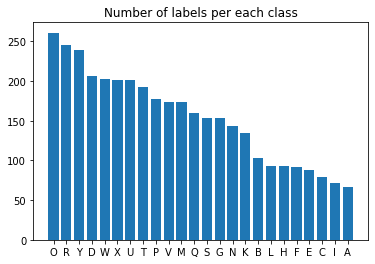
\includegraphics[width=\textwidth]{thesis/images/static_hand_gestures_dataset.png}
    \caption{Class distribution in the static hand gestures dataset.}
    \label{fig:class_distribution_static_hand_gestures}
\end{figure}

\subsubsection{Tests}
In table~\ref{tab:tests_static_hand_gestures} are listed the tests performed to find the best configuration to recognize static hand gestures. ``Not defined'' in the column of ``Number of elements per class'' means that the whole dataset, described in~\ref{ss:dataset_static_gestures}, has been used to train the network
\begin{table}[H]
\begin{tabular}{|c|c|c|}
\hline
\textbf{Test name}          & \textbf{Number of elements per class} & \textbf{Dropout rate} \\ \hline
full\_dataset               & Not defined                           & 0.0                   \\ \hline
full\_dataset\_dropout & Not defined                           & 0.2                   \\ \hline
10\_samples                 & 10                                    & 0.0                   \\ \hline
7\_samples                  & 7                                     & 0.0                   \\ \hline
6\_samples                  & 6                                     & 0.0                   \\ \hline
5\_samples                  & 5                                     & 0.0                   \\ \hline
\end{tabular}
\caption{Training configurations for the static hand gesture classifier.}\label{tab:tests_static_hand_gestures}
\end{table}
I mainly focused on finding the minimum amount of samples in order to obtain a good accuracy and a short training time. 

\subsubsection{Results}
\begin{table}[H]
\begin{tabular}{|c|c|c|c|}
\hline
\textbf{Test name}          & \textbf{Evaluation accuracy} & \textbf{Evaluation loss} & \textbf{Training time} \\ \hline
full\_dataset               & 0.99                         & 0.03                     & 6s 587ms               \\ \hline
full\_dataset\_dropout & 0.99                         & 0.01                     & 38s 769ms              \\ \hline
10\_samples                 & 1                            & 0.02                     & 26s 883ms              \\ \hline
7\_samples                  & 1                            & 0.04                     & 15s 804ms              \\ \hline
6\_samples                  & 1                            & 0.009                    & 31s 839ms              \\ \hline
5\_samples                  & 0.27                         & 2.90                     & 4s 551ms               \\ \hline
\end{tabular}
\caption{Results for training the static hand gesture recognizer.}
\label{tab:result_static_hand_gestures}
\end{table}

\begin{figure}[H]
     \centering
     \begin{subfigure}[b]{0.45\textwidth}
         \centering
         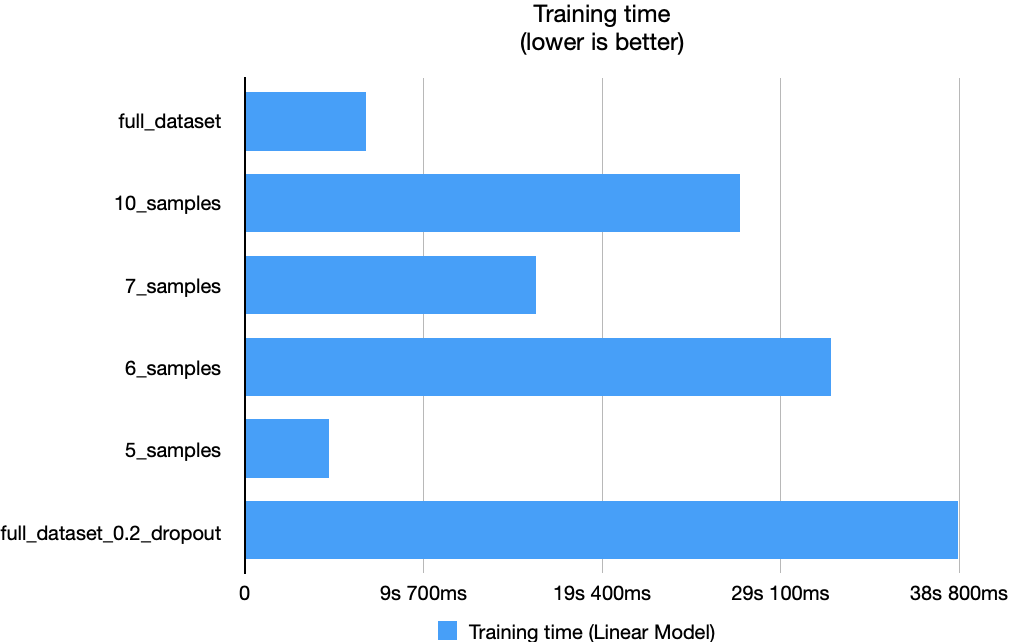
\includegraphics[width=\textwidth]{thesis/images/training_time_hand_gestures.png}
         \caption{Training time in tests static hand gestures.}
         \label{fig:training_time_static_hand_gestures}
     \end{subfigure}
     \hfill
     \begin{subfigure}[b]{0.45\textwidth}
         \centering
         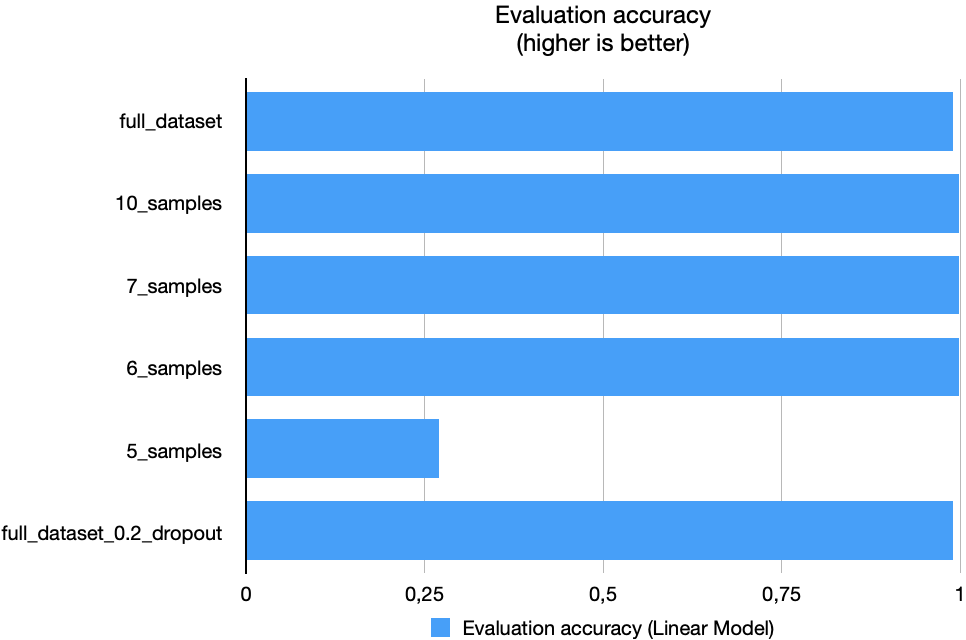
\includegraphics[width=\textwidth]{thesis/images/evaluation_accuracy_static_hand_gestures.png}
         \caption{Accuracy in tests static hand gestures.}
         \label{fig:evaluation_accuracy_static_hand_gestures}
     \end{subfigure}
     \hfill
     \begin{subfigure}[b]{0.45\textwidth}
         \centering
         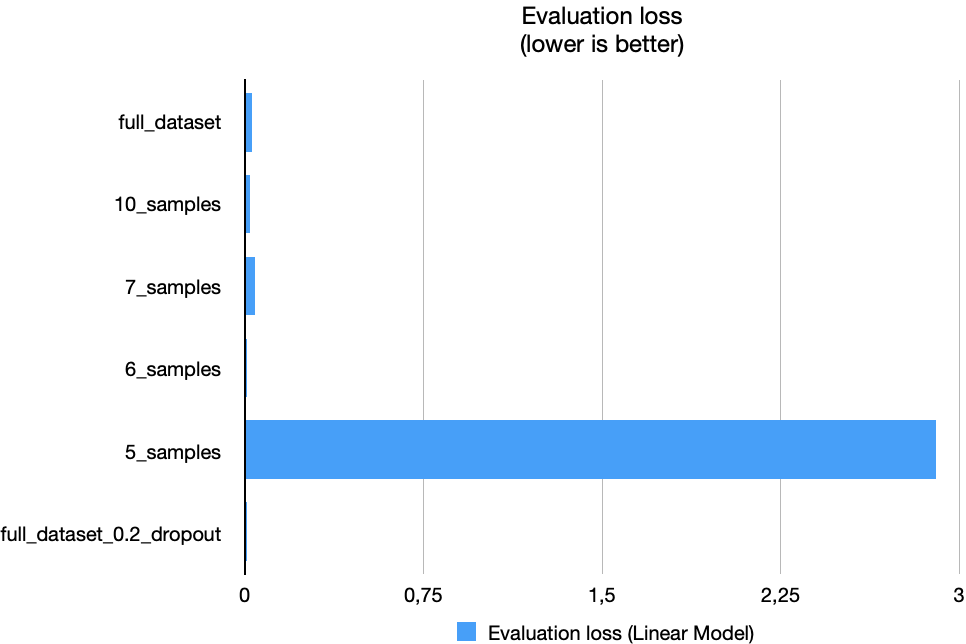
\includegraphics[width=\textwidth]{thesis/images/evaluation_loss_static_hand_gestures.png}
         \caption{Loss in tests static hand gestures.}
         \label{fig:evaluation_loss_static_hand_gestures.}
     \end{subfigure}
        \caption{Results graphs for the training of the static hand gesture recognizer}
        \label{fig:results_graphs_static_hand_gestures}
\end{figure}

\subsection{Dynamic hand gesture}

\subsubsection{Dataset}
Two datasets have been used:
\begin{itemize}
    \item \textbf{five\_fingers}: in this dataset the history of the tip of every finger has been saved. There are $461$ elements with a total size of $1.1MB$. Its class distribution is shown in figure~\ref{fig:class_distribution_dynamic_hand_gestures_five_fingers};
    \item \textbf{one\_finger}: in this dataset only the history of the tip of the index finger has been saved. There are $994$ elements with a total size of $423KB$. Its class distribution is shown in figure~\ref{fig:class_distribution_dynamic_hand_gestures_one_finger}.
\end{itemize}

\begin{figure}[H]
    \centering
    \begin{subfigure}[b]{0.45\textwidth}
        \centering
        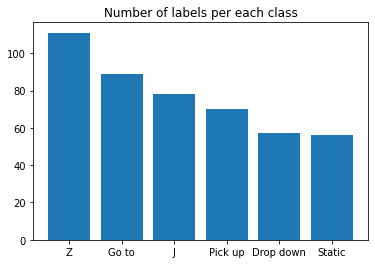
\includegraphics[width=\textwidth]{thesis/images/dynamic_hand_gestures_five_fingers.png}
        \caption{Class distribution in the dynamic hand gestures dataset with five fingers.}
        \label{fig:class_distribution_dynamic_hand_gestures_five_fingers}
    \end{subfigure}
    \hfill
    \begin{subfigure}[b]{0.45\textwidth}
        \centering
        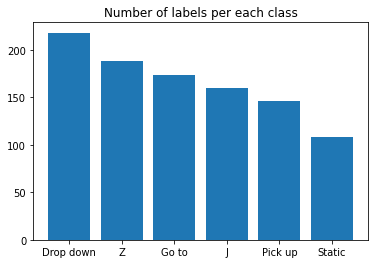
\includegraphics[width=\textwidth]{thesis/images/dynamic_hand_gestures_one_finger.png}
        \caption{Class distribution in the dynamic hand gestures dataset with one finger.}
        \label{fig:class_distribution_dynamic_hand_gestures_one_finger}
    \end{subfigure}
    \caption{Class distribution in the dynamic hand gestures datasets.}
    \label{fig:my_label}
\end{figure}

\subsubsection{Tests}
\begin{table}[H]
\begin{tabular}{|c|c|c|c|}
\hline
\textbf{Test name} & \textbf{Dataset} & \textbf{Network type} & \textbf{Number of elements per class} \\ \hline
full\_dataset      & five\_fingers    & feed\_forward         & Not defined                           \\ \hline
50\_samples        & five\_fingers    & feed\_forward         & 50                                    \\ \hline
10\_samples        & five\_fingers    & feed\_forward         & 10                                    \\ \hline
full\_dataset      & five\_fingers    & lstm                  & Not defined                           \\ \hline
50\_samples        & five\_fingers    & lstm                  & 50                                    \\ \hline
10\_samples        & five\_fingers    & lstm                  & 10                                    \\ \hline
full\_dataset      & one\_finger      & feed\_forward         & Not defined                           \\ \hline
50\_samples        & one\_finger      & feed\_forward         & 50                                    \\ \hline
10\_samples        & one\_finger      & feed\_forward         & 10                                    \\ \hline
\end{tabular}
\caption{Training configurations for the dynamic hand gesture classifier.}
\label{tab:tests_dynamic_hand_gestures}
\end{table}

\subsubsection{Results}
\begin{table}[H]
\resizebox{\textwidth}{!}{%
\begin{tabular}{|c|c|c|c|c|c|}
\hline
\textbf{Test name} & \textbf{Dataset} & \textbf{Network type} & \textbf{Evaluation accuracy} & \textbf{Evaluation loss} & \textbf{Training time} \\ \hline
full\_dataset      & five\_fingers    & feed\_forward         & 0.98                         & 0.02                     & 19s 878ms              \\ \hline
50\_samples        & five\_fingers    & feed\_forward         & 0.97                         & 0.04                     & 14s 558ms              \\ \hline
10\_samples        & five\_fingers    & feed\_forward         & 0.77                         & 1,27                     & 16s 970ms              \\ \hline
full\_dataset      & five\_fingers    & lstm                  & 0.98                         & 0.01                     & 22s 110ms              \\ \hline
50\_samples        & five\_fingers    & lstm                  & 0.97                         & 0.03                     & 24s 161ms              \\ \hline
10\_samples        & five\_fingers    & lstm                  & 0.66                         & 0.95                     & 14s 798ms              \\ \hline
full\_dataset      & one\_finger      & feed\_forward         & 0.93                         & 0.21                     & 38s 749ms              \\ \hline
50\_samples        & one\_finger      & feed\_forward         & 0.95                         & 0.26                     & 42s 535ms              \\ \hline
10\_samples        & one\_finger      & feed\_forward         & 0                            & 1.82                     & 2s 622ms               \\ \hline
\end{tabular}%
}
\caption{Results for training the dynamic hand gesture recognizer.}
\label{tab:result_dynamic_hand_gestures}
\end{table}

\begin{figure}[H]
     \centering
     \begin{subfigure}[b]{0.45\textwidth}
         \centering
         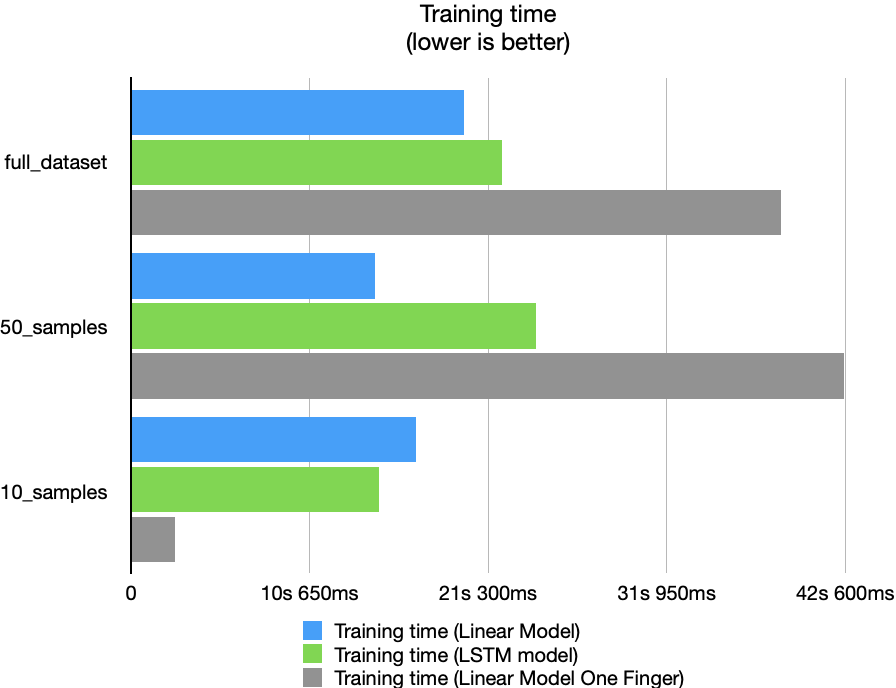
\includegraphics[width=\textwidth]{thesis/images/training_time_dynamic_hand_gestures.png}
         \caption{Training time in tests dynamic hand gestures.}
         \label{fig:training_time_static_hand_gestures}
     \end{subfigure}
     \hfill
     \begin{subfigure}[b]{0.45\textwidth}
         \centering
         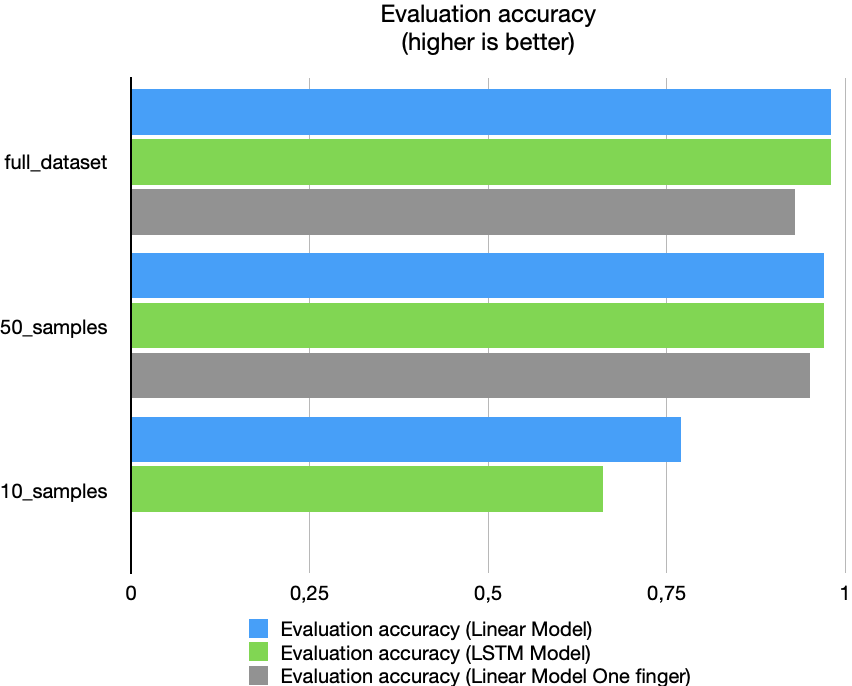
\includegraphics[width=\textwidth]{thesis/images/evaluation_accuracy_dynamic_hand_gestures.png}
         \caption{Accuracy in tests dynamic hand gestures.}
         \label{fig:evaluation_accuracy_static_hand_gestures}
     \end{subfigure}
     \hfill
     \begin{subfigure}[b]{0.45\textwidth}
         \centering
         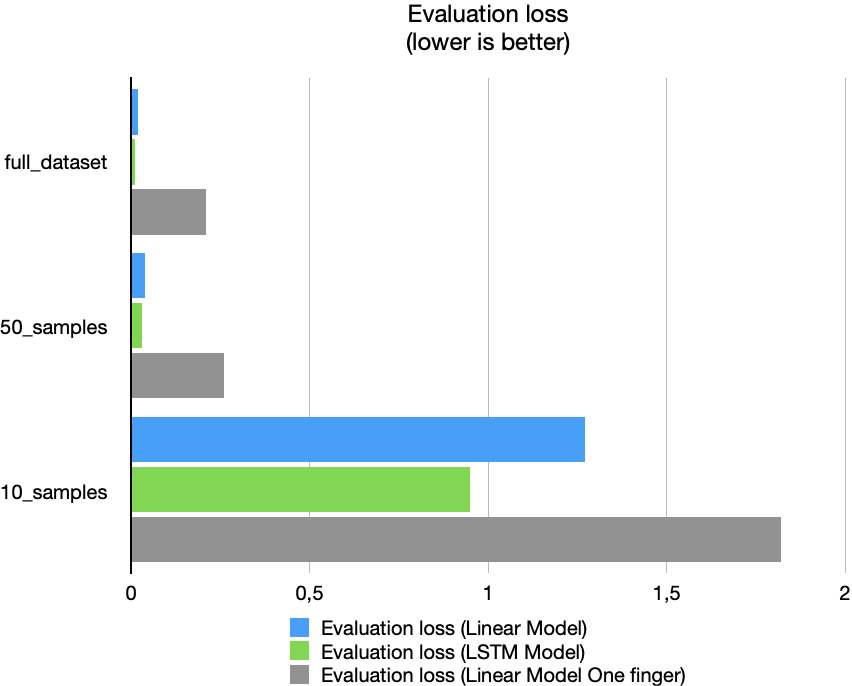
\includegraphics[width=\textwidth]{thesis/images/evaluation_loss_dynamic_hand_gestures.png}
         \caption{Loss in tests dynamic hand gestures.}
         \label{fig:evaluation_loss_static_hand_gestures.}
     \end{subfigure}
        \caption{Results graphs for the training of the dynamic hand gesture recognizer}
        \label{fig:results_graphs_static_hand_gestures}
\end{figure}

\end{document}
